% -------------------------------------------------------
% This plot is from DefElement (https://defelement.com)
% and is available under a Creative Commons Attribution
% 4.0 International (CC BY 4.0) license:
% https://creativecommons.org/licenses/by/4.0/
% -------------------------------------------------------
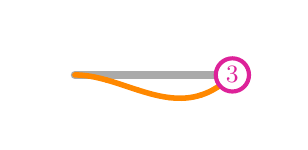
\begin{tikzpicture}[x=0.2mm,y=0.2mm]
\definecolor{color0}{HTML}{AAAAAA}
\definecolor{color1}{HTML}{FF8800}
\definecolor{color2}{HTML}{DD2299}
\clip (0,0) rectangle (160,60);
\draw[color0,line width=3pt,line cap=round](30.0,30.0) -- (130.0,30.0);
\draw[color1,line cap=round,line width=2pt] (30.0,30.0) .. controls (36.666666666666664,30.0) and (43.333333333333336,28.666666666666668) .. (50.0,26.8);
\draw[color1,line cap=round,line width=2pt] (50.0,26.8) .. controls (56.66666666666667,24.933333333333334) and (63.33333333333333,22.53333333333333) .. (70.0,20.4);
\draw[color1,line cap=round,line width=2pt] (70.0,20.4) .. controls (76.66666666666666,18.266666666666666) and (83.33333333333334,16.4) .. (90.0,15.599999999999998);
\draw[color1,line cap=round,line width=2pt] (90.0,15.599999999999998) .. controls (96.66666666666666,14.8) and (103.33333333333333,15.066666666666663) .. (110.0,17.2);
\draw[color1,line cap=round,line width=2pt] (110.0,17.2) .. controls (116.66666666666667,19.333333333333336) and (123.33333333333333,23.333333333333336) .. (130.0,30.0);
\draw[color2,fill=white,line width=1.5pt] (130.0,30.0)circle (6pt);
\node[anchor=center] at (130.0,30.0) {\small\color{color2}3};
\end{tikzpicture}